%%%%%%%%%%%%%%%%%%%%%%%%%%%%%%%%%%%%%%%%%%%%%%%%%%%%%%%%%%%%%
% Use the BCUReport class
%%%%%%%%%%%%%%%%%%%%%%%%%%%%%%%%%%%%%%%%%%%%%%%%%%%%%%%%%%%%%
\documentclass{BCUReport}
\usepackage{float}
\usepackage{amsmath}
\usepackage{url}
\usepackage{hyperref}
\usepackage{siunitx}
\usepackage{enumitem}
\usepackage{pdfpages}

%%%%%%%%%%%%%%%%%%%%%%%%%%%%%%%%%%%%%%%%%%%%%%%%%%%%%%%%%%%%%
% Enter document details here
%%%%%%%%%%%%%%%%%%%%%%%%%%%%%%%%%%%%%%%%%%%%%%%%%%%%%%%%%%%%%
\author{Harvey Fretwell}
\studentid{20113452}
\title{Live Sound Reinforcement 2}
\module{DIG6108}
\course{Sound Engineering and Production}
\date{\today}
\wordcount{\todo{Need to add word count}}

%%%%%%%%%%%%%%%%%%%%%%%%%%%%%%%%%%%%%%%%%%%%%%%%%%%%%%%%%%%%%
% Define acronyms
%%%%%%%%%%%%%%%%%%%%%%%%%%%%%%%%%%%%%%%%%%%%%%%%%%%%%%%%%%%%%
% Acronyms are defined using the \newacronym command.
%  * The first argument is the name of the acronym.
%  * The second argument is the abbreviated form.
%  * The third argument is the full form.
\newacronym{spl}{SPL}{Sound Pressure Level}
\newacronym{vap}{VAP}{Vehicle Access Point}
\newacronym{pap}{PAP}{Pedestrian Access Point}
\newacronym{foh}{FOH}{Front of House}
\glsfindwidesttoplevelname % Leave this here so the list of acronyms looks nice

%%%%%%%%%%%%%%%%%%%%%%%%%%%%%%%%%%%%%%%%%%%%%%%%%%%%%%%%%%%%%
% Begin the document.
%%%%%%%%%%%%%%%%%%%%%%%%%%%%%%%%%%%%%%%%%%%%%%%%%%%%%%%%%%%%%
\begin{document}

%%%%%%%%%%%%%%%%%%%%%%%%%%%%%%%%%%%%%%%%%%%%%%%%%%%%%%%%%%%%%
% Create title page.
%%%%%%%%%%%%%%%%%%%%%%%%%%%%%%%%%%%%%%%%%%%%%%%%%%%%%%%%%%%%%
\maketitle

%%%%%%%%%%%%%%%%%%%%%%%%%%%%%%%%%%%%%%%%%%%%%%%%%%%%%%%%%%%%%
% Set initial page numbering to be lower case roman numerals and include the contents of the preamble.tex file.
%%%%%%%%%%%%%%%%%%%%%%%%%%%%%%%%%%%%%%%%%%%%%%%%%%%%%%%%%%%%%
% Leave this here to use roman numeral page numbering for the preamble.
\pagenumbering{roman}

% The Abstract
\begin{abstract}
	In this comprehensive report, the planning and design of a large-scale outdoor music event is detailed. The project involves utilising tools such as ArrayCalc to create a bespoke speaker system tailored to the specific needs of a specified band. The careful selection of equipment is justified through thorough research, considering technical specifications and industry standards. The system integration is outlined with a focus on advanced audio networking protocols. Power requirements are calculated using excel, and environmentally friendly solutions and provided. The report culminates in a thorough risk assessment using Microsoft Word, ensuring all potential hazards are identified and addressed. Overall, this project not only delves into the technical intricacies of event planning but also prioritises a seamless and optimal experience for both performers and audiences.
\end{abstract}

% ToC and lists of figures/tables etc.
\tableofcontents
\listoffigures
\listoftables
\listofacronyms
\clearpage

%%%%%%%%%%%%%%%%%%%%%%%%%%%%%%%%%%%%%%%%%%%%%%%%%%%%%%%%%%%%%
% Set page numbering back to normal numbers and include each individual chapter.
%%%%%%%%%%%%%%%%%%%%%%%%%%%%%%%%%%%%%%%%%%%%%%%%%%%%%%%%%%%%%
% Leave these here to change back to normal page numbering and add some nice headers to the pages.
\pagenumbering{arabic}
\pagestyle{headings}

\section{Introduction}
    This report demonstrates the planning of a hypothetical large-scale (50,000 - 100,000 people) outdoor music event, including the entire event setup and system design for a specified band. Utilizing ArrayCalc to design a speaker system for the event. Equipment will be carefully chosen based on the band's requirements and comparative research. Excel will be employed to create a comprehensive patch sheet, outline the system integration and calculate power requirements. Finally, a risk assessment will be formulated using Microsoft Word to identify necessary precautions.

    \subsection{Aims}
    The aim of this report is to plan and design various aspects of a large-scale outdoor music festival. This report will explain the rationale behind the selection of specific equipment and decisions over alternatives, aiming to craft a detailed design that ensures an optimal experience.
    
    \subsection{Objectives}
        \begin{itemize}
            \item Specify technical requirements for the event (such as microphones, desks, stage boxes, amplifiers and loudspeakers), tailoring the equipment for a specified band and venue.
            \item Design a bespoke speaker system for an outdoor venue and calculate the \gls{spl}, taking health and safety requirements into consideration.
            \item Justify equipment choices through meticulous research and evaluation of technical specifications, bearing in mind the band's equipment specifications.
            \item Identify and compare suitable audio networking solutions and protocols, while integrating redundancy within the system integration plan.
            \item Calculate power requirements, choose appropriate generators, and explore eco-friendly options.
        \end{itemize}
    
\section{Event Planning}
    \subsection{Venue}

        \begin{figure}[H]
            \centering
            \includegraphics[width=\textwidth]{Images/festival_maps.jpg}
            \caption{Map of the surrounding area}
            \label{fig:festival_map}
        \end{figure}
        
        The Town Moor in Newcastle Upon Tyne was selected for its UK city setting, offering approximately 1,000 acres of open space to accommodate a crowd of 50,000 to 100,000 people. Situated near a well-known brewery and various amenities, this centrally located area, which has previously hosted one of Europe's largest travelling fairs, fulfils the project requirements.
        
        \begin{figure}[H]
            \centering
            \includegraphics[width=\textwidth]{Images/festival_expand.jpg}
            \caption{Satellite image with city centre (purple), and festival location (green)}
            \label{fig:festival_expand}
        \end{figure}

        Given the proximity to busy A roads and motorways, sound pollution is anticipated to be partially masked in this area. The vast size of the park should contain most of the pollution. Strategies, including minimizing rear-firing through techniques like end-fire for a cardioid sub frequency response, will be explored. The festival's location and direction are expected to aid in dissipating audio across extended sections of the moor.
        
        \begin{figure}[H]
            \centering
            \includegraphics[width=\textwidth]{Images/festival_vap_pap.jpg}
            \caption{Festival \acrshort{vap} [ small (yellow) medium (orange) and large (red) ] and \acrshort{pap} (black)}
            \label{fig:festival_vap_pap}
        \end{figure}

        Figure \ref{fig:festival_vap_pap} shows the \acrfull{vap} with large, medium and small sized vehicle routes for setup and staff access. \acrfull{pap} indicates the access routes for pedestrians entering the festival area.

        \begin{figure}[H]
            \centering
            \includegraphics[width=\textwidth]{Images/festival_close_up.jpg}
            \caption{Festival layout with toilets (light blue strips), vendor booths (orange strips), medical tents (red), entrance/exit (red PA / running man), staff tents (dark blue), stage (purple)}
            \label{fig:festival_close_up}
        \end{figure}

        Figure \ref{fig:festival_close_up} shows a rough guide of various amenities, with measurements calculated as shown in Table \ref{tab:amenities_calcs} (some measurements have been rounded up for simplicity in calculations and to give room for error).

        \begin{longtable}{|p{1.5cm}|p{14cm}|}
            \hline
            \textbf{Item} & \textbf{Calculations} \\
            \hline
            \endhead % header for subsequent pages
            Total Area & To comply with fire and safety regulations, the festival's total area must be carefully allocated. According to \citet{mmontgomery2018}, the following considerations should be taken into account:
        
            \begin{itemize}
                \item At least 200 square meters must be set aside for the staging area. The requested area is $\SI{20}{\metre} \times \SI{30}{\metre}$, which equals \SI{600}{\metre\squared}.
                \item At least \SI{500}{\metre\squared} should be reserved for vendor booths, staff, security, and medical personnel. Scaling this by the same factor as the staging area, we get $3 \times \SI{500}{\metre\squared} \approx \SI{1500}{\metre\squared}$, divided into approximately \SI{500}{\metre\squared} each for vendor booths, staff \& security, and medical personnel.
                \item Under fire and health safety regulations, the remaining area should provide 2 people per square meter. For the main festival standing audience (at full capacity), an area of \SI{50000}{\metre\squared} will be required.
                \item For a moving queuing system, the guidance suggests 4 people per square meter. Therefore, an area of \SI{25000}{\metre\squared} will be allocated for the queuing audience (at full capacity).
            \end{itemize} \\
            \hline
            Exits & 
                \citet{hmgovernment2007} states that the risk of outdoor fires is typically considered lower than indoor fires due to reduced susceptibility to smoke and heat, and outdoor escape routes are less likely to be obstructed. 
    
                \textbf{Risk to Exit Time:}
                \[
                    \begin{aligned}
                          \text{High: }&   &<& \SI{5}{\minute}\\
                        \text{Normal: }& 5 &<& \SI{10}{\minute}\\
                           \text{Low: }&   &>& \SI{10}{\minute}
                    \end{aligned}
                \]
    
                \textbf{Appropriate Flow Rate for Outdoor Standing Events:}
                109 people per meter of escape width, per minute.
    
                \textbf{Total Exit Width Calculation:}
                \[
                    \text{Total Exit Width} = \frac{\text{Number of People}}{\text{Flow Rate} \times \text{Escape Time}} \approx \SI{92}{\metre}
                \]
    
                \textbf{Minimum Exit Size:}
                1.09 meters, adjustable for larger venues.
    
                To determine the required exit width for a venue, the formula considers both the nominal exits needed and an additional exit to account for potential blockages during a fire event:
                \[
                    \text{Total Exits} = \text{Nominal Exits} + 1
                \]
    
                For a given exit width of 7 meters, the nominal exits required can be calculated using the formula:
                \[
                    \begin{aligned}
                    \text{Nominal Exits} &= \frac{\text{Total Exit Width}}{\text{Exit Width per Exit}}\\
                                         &\approx 12 \text{ nominal exits}
                    \end{aligned}
                \]
    
                Additionally, the total capacity of the exits can be determined by multiplying the flow rate of 109 persons per minute by the total escape width of 92 meters:
                \[
                    \begin{aligned}
                    \text{Total Capacity} &= \text{Flow Rate} \times \text{Total Escape Width}\\
                                          &\approx 10,000 \text{ persons per minute}
                    \end{aligned}
                \]
    
                To estimate the number of people leaving within a given time frame (e.g., 10 minutes), the total capacity is further multiplied by the time:
                \[
                    \begin{aligned}
                    \text{Number of People Leaving}
                    &= \text{Total Capacity} \times \text{Time}\\
                    &\approx 100,000 \text{ people for 10 minutes}
                    \end{aligned}
                \]
    
                Therefore, a total of 13 exits with a width of 7 meters will be required.
            \\
            \hline
            Vendor Booths &
                According to information from \citet{jjones2023}, food trucks are typically \SI{5}{\metre} long by \SI{2}{\metre} wide, but can range from \SI{3}{\metre} to \SI{8}{\metre} long by \SI{2}{\metre} to \SI{3}{\metre} wide. Let's assume we have $\SI{5}{\metre} \times \SI{2}{\metre}$ trucks, which equals \SI{10}{\metre\squared}. With the available area of \SI{500}{\metre\squared}, we can accommodate 50 vendor booths $(\SI{500}{\metre\squared} \div \SI{10}{\metre\squared})$.
            \\
            \hline
            Medical Regulations &
                Based on first aid cover guidelines from \citet{sja2023} and ambulance size specifications from \citet{nhs-ambulance-specs}, the medical regulations can be calculated as follows:

                First aid cover:
                \begin{itemize}
                    \item 2 first aiders per 1,000 people = 200 first aiders
                    \begin{itemize}
                        \item 152 first aiders in and around the crowd
                        \item 48 in tents (6 per tent for 8 tents)
                    \end{itemize}
                    \item Standard first aid tent size = $\SI{8}{\metre} \times \SI{4}{\metre} = \SI{32}{\metre\squared}$
                \end{itemize}

                Ambulance size = $\SI{2.45}{metre} \times \SI{6.95}{\metre} \approx \SI{18}{\metre\squared}$.

                According to \citet{hmas-festivals}, for festivals with 4,000 people, 1 ambulance or response vehicle is recommended, therefore 100,000 people require 25 ambulances or response vehicles.
            \\
            \hline
            Toilets &
                For a large music events featuring alcohol, food, and drinks, the required toilets can be calculated using the following guidelines from \citet{lsharp2023} and \citet{andyloos2015}:

                \begin{itemize}
                    \item Women: 1 portaloo per 75 people
                    \item Men: 1 portaloo per 400 people
                    \item Men: 1 urinal per 100 people
                \end{itemize}
                
                Taking into account the percentage split of men to women at festivals (e.g., at Latitude Festival, the split was 40\% women and 60\% men \citep{aawbi2019}), therefore, considering an example with 100,000 attendees, the minimum required toilets would be:
                
                \begin{itemize}
                    \item Total minimum: 1000
                    \item Women's toilets: 534
                    \item Men's toilets: 150
                    \item Urinals: 600
                \end{itemize}
                
                Therefore, based on standard portaloo sizes of $\SI{1.1}{\metre} \times \SI{1.2}{\metre}$, arranged in rows of 42 toilets per row, with pairs of rows back to back, this requires 12 pairs of rows. Taking up a total of \SI{1320}{\metre\squared}:

                \[
                    \begin{aligned}
                    \SI{1.1}{\metre} \times \SI{1.2}{\metre} &= \SI{1.32}{\metre\squared} &\text{ for 1 portaloo}\\
                    \SI{1.32}{\metre\squared} \times 1000 &= \SI{1320}{\metre\squared} &\text{ for 1000 portaloos}
                    \end{aligned}
                \]
            \\
            \hline
            FOH and Backstage Areas &
                Tents with the dimensions of $\SI{20}{\metre} \times \SI{10}{\metre}$ will be provided for each: FOH ($\approx \SI{120}{\metre}$ away from stage), stage left and stage right. A backstage truck provides a $\SI{50}{\metre} \times \SI{10}{\metre}$ area for artists and backline tech.
            \\
            \hline

            \caption{Calculation of all amenities}
            \label{tab:amenities_calcs}
        \end{longtable}

    \subsection{Regulations and Guidance}
        During indoor rock concerts, sound levels typically surpass 100 dBs for extended periods, with peaks reaching 130 dB. However, there's limited data on sound exposure at outdoor music festivals, particularly those spanning multiple stages across several days \citep{rmbrecht2023}.

        As the LAeq will exceed \SI{96}{\dB}, tickets, advertising and notices at entry points will advise the audience of the risk to their hearing in advance \citep{hse-event-safety-noise}. Hearing protection will be provided on the door especially as younger kids have sensitive hearing and anything over \SI{85}{\dB} can cause damage \citep{rmbrecht2023}.

        \citet{hse-event-safety-noise} states that the continuous A-weighted \acrshort{spl} over an event should not exceed \SI{107}{\dB} and the C-weighted peak \acrshort{spl} should not exceed \SI{130}{\dB} within the audience. Therefore, during soundcheck and at intervals throughout the festival, the \acrshort{foh} will perform regular \acrshort{spl} checks. The audience to loudspeaker separation distance should also exceed \SI{1}{\metre} to help reduce the peak levels within the area.

\section{Band Planning}
    \subsection{General Information}

    \subsection{Patch Sheet}

    \subsection{Riser Requirements}

    \subsection{Monitor Requirements}

\section{System Design}
    \note{
        Add stuff here.
    }
    
    \subsection{System Overview}
        
    \subsection{Speaker System}
    The \acrshort{spl} mapping of the system can be seen in Table \ref{tab:spl_mapping}; showing the highest, lowest, standard deviation and average \acrshort{spl}.

    \subsubsection{SPL Mapping}
        \begin{longtable}[H]{|c|c|c|c|c|c|}
            \hline
            \multicolumn{1}{|c|}{\textbf{Freq}} &
            \multicolumn{1}{c|}{\textbf{Screenshot}} &
            \multicolumn{1}{c|}{\textbf{\begin{tabular}[c]{@{}c@{}}High\\ SPL\end{tabular}}} &
            \multicolumn{1}{c|}{\textbf{\begin{tabular}[c]{@{}c@{}}Low\\ SPL\end{tabular}}} &
            \multicolumn{1}{c|}{\textbf{\begin{tabular}[c]{@{}c@{}}Std\\ Dev\end{tabular}}} &
            \textbf{\begin{tabular}[c]{@{}c@{}}Avg.\\ SPL\end{tabular}} \\ \hline
            \endfirsthead
            %
            \endhead
            %
            \multicolumn{6}{|c|}{\textbf{Sub Array Only (all other sources muted)}}                                                                           \\ \hline
            \multicolumn{1}{|c|}{\SI{50}{\Hz}}  & \multicolumn{1}{c|}{\includegraphics[width=0.5\textwidth]{Images/spl_plot_50hz_subs.png}}  & \multicolumn{1}{c|}{\SI{119.5}{\dB}} & \multicolumn{1}{c|}{\SI{84}{\dB}}  & \multicolumn{1}{c|}{\SI{25.1}{\dB}} & \SI{101.8}{\dB} \\ \hline
            \multicolumn{1}{|c|}{\SI{100}{\Hz}} & \multicolumn{1}{c|}{\includegraphics[width=0.5\textwidth]{Images/spl_plot_100hz_subs.png}} & \multicolumn{1}{c|}{\SI{113.5}{\dB}} & \multicolumn{1}{c|}{\SI{78}{\dB}}  & \multicolumn{1}{c|}{\SI{25.1}{\dB}} & \SI{95.8}{\dB} \\ \hline
            \multicolumn{6}{|c|}{\textbf{Full System}}                                                                                                        \\ \hline
            \multicolumn{1}{|c|}{\SI{50}{\Hz}}  & \multicolumn{1}{c|}{\includegraphics[width=0.5\textwidth]{Images/spl_plot_50hz_all.png}}   & \multicolumn{1}{c|}{\SI{120.0}{\dB}} & \multicolumn{1}{c|}{\SI{96}{\dB}}  & \multicolumn{1}{c|}{\SI{17.0}{\dB}} & \SI{108.0}{\dB} \\ \hline
            \multicolumn{1}{|c|}{\SI{100}{\Hz}} & \multicolumn{1}{c|}{\includegraphics[width=0.5\textwidth]{Images/spl_plot_100hz_all.png}}  & \multicolumn{1}{c|}{\SI{121.8}{\dB}} & \multicolumn{1}{c|}{\SI{102}{\dB}} & \multicolumn{1}{c|}{\SI{14.0}{\dB}} & \SI{111.9}{\dB} \\ \hline
            \multicolumn{1}{|c|}{\SI{500}{\Hz}} & \multicolumn{1}{c|}{\includegraphics[width=0.5\textwidth]{Images/spl_plot_500hz.png}}      & \multicolumn{1}{c|}{\SI{117.9}{\dB}} & \multicolumn{1}{c|}{\SI{96}{\dB}}  & \multicolumn{1}{c|}{\SI{15.5}{\dB}} & \SI{107.0}{\dB} \\ \hline
            \multicolumn{1}{|c|}{\SI{1}{\kHz}}  & \multicolumn{1}{c|}{\includegraphics[width=0.5\textwidth]{Images/spl_plot_1khz.png}}       & \multicolumn{1}{c|}{\SI{116.1}{\dB}} & \multicolumn{1}{c|}{\SI{90}{\dB}}  & \multicolumn{1}{c|}{\SI{18.5}{\dB}} & \SI{103.1}{\dB} \\ \hline
            \multicolumn{1}{|c|}{\SI{2}{\kHz}}  & \multicolumn{1}{c|}{\includegraphics[width=0.5\textwidth]{Images/spl_plot_2khz.png}}       & \multicolumn{1}{c|}{\SI{116.1}{\dB}} & \multicolumn{1}{c|}{\SI{90}{\dB}}  & \multicolumn{1}{c|}{\SI{18.5}{\dB}} & \SI{103.1}{\dB} \\ \hline
            \multicolumn{1}{|c|}{\SI{5}{\kHz}}  & \multicolumn{1}{c|}{\includegraphics[width=0.5\textwidth]{Images/spl_plot_5khz.png}}       & \multicolumn{1}{c|}{\SI{116.6}{\dB}} & \multicolumn{1}{c|}{\SI{96}{\dB}}  & \multicolumn{1}{c|}{\SI{14.6}{\dB}} & \SI{106.3}{\dB} \\ \hline
            \multicolumn{1}{|c|}{\SI{10}{\kHz}} & \multicolumn{1}{c|}{\includegraphics[width=0.5\textwidth]{Images/spl_plot_10khz.png}}      & \multicolumn{1}{c|}{\SI{119.1}{\dB}} & \multicolumn{1}{c|}{\SI{72}{\dB}}  & \multicolumn{1}{c|}{\SI{33.3}{\dB}} & \SI{95.6}{\dB} \\ \hline
            \multicolumn{1}{|c|}{Pink}          & \multicolumn{1}{c|}{\includegraphics[width=0.5\textwidth]{Images/spl_plot_pink_none.png}}  & \multicolumn{1}{c|}{\SI{116.4}{\dB}} & \multicolumn{1}{c|}{\SI{96}{\dB}}  & \multicolumn{1}{c|}{\SI{14.4}{\dB}} & \SI{106.2}{\dB} \\ \hline
            
            \caption{SPL Mapping}
            \label{tab:spl_mapping}
        \end{longtable}

    \subsubsection{Parts List}
        The parts list for the system is specified in Table \ref{tab:parts_list}.

        \begin{longtable}[H]{|llll|}
            \hline
            \multicolumn{1}{|l|}{\textbf{Origin}} & \multicolumn{1}{l|}{\textbf{d\&b Part no.}} & \multicolumn{1}{l|}{\textbf{Total}} & \textbf{Part name}         \\ \hline
            \endfirsthead
            %
            \endhead
            %
            \multicolumn{4}{|l|}{\textbf{Main}}                                                                                                                    \\ \hline
            \multicolumn{4}{|c|}{GSL}                                                                                                                              \\ \hline
            \multicolumn{1}{|l|}{--}              & \multicolumn{1}{l|}{Z0751}                  & \multicolumn{1}{l|}{44}             & GSL12                      \\ \hline
            \multicolumn{1}{|l|}{--}              & \multicolumn{1}{l|}{Z5706}                  & \multicolumn{1}{l|}{4}              & Hoist chain 4t             \\ \hline
            \multicolumn{1}{|l|}{--}              & \multicolumn{1}{l|}{Z5707}                  & \multicolumn{1}{l|}{2}              & SL Aiming plate (optional) \\ \hline
            \multicolumn{1}{|l|}{--}              & \multicolumn{1}{l|}{Z5708}                  & \multicolumn{1}{l|}{2}              & GSL Flying frame set       \\ \hline
            \multicolumn{4}{|l|}{\textbf{Outfill L}}                                                                                                               \\ \hline
            \multicolumn{4}{|c|}{GSL}                                                                                                                              \\ \hline
            \multicolumn{1}{|l|}{--}              & \multicolumn{1}{l|}{Z0751}                  & \multicolumn{1}{l|}{16}             & GSL12                      \\ \hline
            \multicolumn{1}{|l|}{--}              & \multicolumn{1}{l|}{Z5704}                  & \multicolumn{1}{l|}{1}              & GSL Compression set        \\ \hline
            \multicolumn{1}{|l|}{--}              & \multicolumn{1}{l|}{Z5706}                  & \multicolumn{1}{l|}{2}              & Hoist chain 4t             \\ \hline
            \multicolumn{1}{|l|}{--}              & \multicolumn{1}{l|}{Z5707}                  & \multicolumn{1}{l|}{1}              & SL Aiming plate (optional) \\ \hline
            \multicolumn{1}{|l|}{--}              & \multicolumn{1}{l|}{Z5708}                  & \multicolumn{1}{l|}{1}              & GSL Flying frame set       \\ \hline
            \multicolumn{4}{|l|}{\textbf{Outfill R}}                                                                                                               \\ \hline
            \multicolumn{4}{|c|}{GSL}                                                                                                                              \\ \hline
            \multicolumn{1}{|l|}{--}              & \multicolumn{1}{l|}{Z0751}                  & \multicolumn{1}{l|}{16}             & GSL12                      \\ \hline
            \multicolumn{1}{|l|}{--}              & \multicolumn{1}{l|}{Z5704}                  & \multicolumn{1}{l|}{1}              & GSL Compression set        \\ \hline
            \multicolumn{1}{|l|}{--}              & \multicolumn{1}{l|}{Z5706}                  & \multicolumn{1}{l|}{2}              & Hoist chain 4t             \\ \hline
            \multicolumn{1}{|l|}{--}              & \multicolumn{1}{l|}{Z5707}                  & \multicolumn{1}{l|}{1}              & SL Aiming plate (optional) \\ \hline
            \multicolumn{1}{|l|}{--}              & \multicolumn{1}{l|}{Z5708}                  & \multicolumn{1}{l|}{1}              & GSL Flying frame set       \\ \hline
            \multicolumn{4}{|l|}{\textbf{Delay Array L}}                                                                                                           \\ \hline
            \multicolumn{4}{|c|}{KSL}                                                                                                                              \\ \hline
            \multicolumn{1}{|l|}{--}              & \multicolumn{1}{l|}{Z0781}                  & \multicolumn{1}{l|}{14}             & KSL12                      \\ \hline
            \multicolumn{1}{|l|}{--}              & \multicolumn{1}{l|}{Z0785}                  & \multicolumn{1}{l|}{4}              & KSL-SUB                    \\ \hline
            \multicolumn{1}{|l|}{--}              & \multicolumn{1}{l|}{Z5706}                  & \multicolumn{1}{l|}{2}              & Hoist chain 4t             \\ \hline
            \multicolumn{1}{|l|}{--}              & \multicolumn{1}{l|}{Z5707}                  & \multicolumn{1}{l|}{1}              & SL Aiming plate (optional) \\ \hline
            \multicolumn{1}{|l|}{--}              & \multicolumn{1}{l|}{Z5721}                  & \multicolumn{1}{l|}{1}              & KSL Flying frame set       \\ \hline
            \multicolumn{1}{|l|}{--}              & \multicolumn{1}{l|}{Z5724}                  & \multicolumn{1}{l|}{1}              & KSL Compression set        \\ \hline
            \multicolumn{1}{|l|}{--}              & \multicolumn{1}{l|}{Z5747}                  & \multicolumn{1}{l|}{1}              & KSL-SUB Adapter frame      \\ \hline
            \multicolumn{4}{|l|}{\textbf{Delay Array R}}                                                                                                           \\ \hline
            \multicolumn{4}{|c|}{KSL}                                                                                                                              \\ \hline
            \multicolumn{1}{|l|}{--}              & \multicolumn{1}{l|}{Z0781}                  & \multicolumn{1}{l|}{14}             & KSL12                      \\ \hline
            \multicolumn{1}{|l|}{--}              & \multicolumn{1}{l|}{Z0785}                  & \multicolumn{1}{l|}{4}              & KSL-SUB                    \\ \hline
            \multicolumn{1}{|l|}{--}              & \multicolumn{1}{l|}{Z5706}                  & \multicolumn{1}{l|}{2}              & Hoist chain 4t             \\ \hline
            \multicolumn{1}{|l|}{--}              & \multicolumn{1}{l|}{Z5707}                  & \multicolumn{1}{l|}{1}              & SL Aiming plate (optional) \\ \hline
            \multicolumn{1}{|l|}{--}              & \multicolumn{1}{l|}{Z5721}                  & \multicolumn{1}{l|}{1}              & KSL Flying frame set       \\ \hline
            \multicolumn{1}{|l|}{--}              & \multicolumn{1}{l|}{Z5724}                  & \multicolumn{1}{l|}{1}              & KSL Compression set        \\ \hline
            \multicolumn{1}{|l|}{--}              & \multicolumn{1}{l|}{Z5747}                  & \multicolumn{1}{l|}{1}              & KSL-SUB Adapter frame      \\ \hline
            \multicolumn{4}{|l|}{\textbf{Nearfill Array}}                                                                                                          \\ \hline
            \multicolumn{4}{|c|}{V-Series}                                                                                                                         \\ \hline
            \multicolumn{1}{|l|}{--}              & \multicolumn{1}{l|}{Z0515}                  & \multicolumn{1}{l|}{6}              & V8                         \\ \hline
            \multicolumn{1}{|l|}{--}              & \multicolumn{1}{l|}{Z5380}                  & \multicolumn{1}{l|}{2}              & V Flying frame             \\ \hline
            \multicolumn{4}{|l|}{\textbf{Frontfill}}                                                                                                               \\ \hline
            \multicolumn{4}{|c|}{Y-Series}                                                                                                                         \\ \hline
            \multicolumn{1}{|l|}{--}              & \multicolumn{1}{l|}{Z0703}                  & \multicolumn{1}{l|}{4}              & Y10P                       \\ \hline
            \multicolumn{4}{|l|}{\textbf{SUB array}}                                                                                                               \\ \hline
            \multicolumn{4}{|c|}{KSL}                                                                                                                              \\ \hline
            \multicolumn{4}{|c|}{SL-SUB}                                                                                                                           \\ \hline
            \multicolumn{1}{|l|}{--}              & \multicolumn{1}{l|}{Z0760}                  & \multicolumn{1}{l|}{12}             & SL-SUB                     \\ \hline
            \multicolumn{4}{|l|}{\textbf{Devices}}                                                                                                                 \\ \hline
            \multicolumn{1}{|l|}{--}              & \multicolumn{1}{l|}{Z2710}                  & \multicolumn{1}{l|}{44}             & D80                        \\ \hline
            \multicolumn{1}{|l|}{--}              & \multicolumn{1}{l|}{Z2750}                  & \multicolumn{1}{l|}{4}              & D20                        \\ \hline
            \multicolumn{1}{|l|}{--}              & \multicolumn{1}{l|}{Z2850}                  & \multicolumn{1}{l|}{12}             & D40                        \\ \hline
            \multicolumn{1}{|l|}{--}              & \multicolumn{1}{l|}{Z4010}                  & \multicolumn{1}{l|}{2}              & DS10                       \\ \hline
            \multicolumn{1}{|l|}{--}              & \multicolumn{1}{l|}{Z4100}                  & \multicolumn{1}{l|}{2}              & DS100                      \\ \hline
           
            \caption{Parts List}
            \label{tab:parts_list}
        \end{longtable}

    \subsubsection{Rigging Requirements}
        The full rigging requirements are provided at \ref{appendix:speaker_rigging} with the required pick points, loads and dimensions specified.

    \subsubsection{Delay Times}
        Delays are crucial to ensure proper alignment of multiple audio sources. Especially when arrays are distributed across different locations and distances from the audience. To calculate the necessary delay times for each speaker array, trigonometry is employed to account for the varying distances between the individual speaker hangs.

        The time delay ($t$) needed to time-align two speaker systems with positions ($x_1, y_1, z_1$) and ($x_2, y_2, z_2$) can be calculated using the formula:

        \begin{equation}\label{eq:time_delay}
            t = \frac{\sqrt{(x_2 - x_1)^2 + (y_2 - y_1)^2 + (z_2 - z_1)^2}}{v}
        \end{equation}

        where ($v$) is the speed of sound in air.

        To calculate the speed of sound ($v$), the following formula is used:

        \begin{equation}\label{eq:speed_of_sound}
            v = 331.4 \sqrt{1 + \frac{T}{273.15}} + 0.6 \times H
        \end{equation}

        where ($T$) is the temperature in degrees Celsius, and ($H$) is the relative humidity.
        
        \citet{cramer1993} and \citet{picard2008} demonstrates equations that includes the altitude (Equation \ref{eq:complex_speed_of_sound}). Using the altitude value, the air pressure is calculated with the barometric formula (Equation \ref{eq:barometric_formula}):

        \begin{equation}\label{eq:barometric_formula}
            P = P_0 e^{-\frac{gM(h - h_0)}{RT}}
        \end{equation}
            
        Where:
        \begin{itemize}
            \item $h$ is the altitude at which we want to calculate the pressure, expressed in meters.
            \item $P$ is the air pressure at altitude $h$.
            \item $P_0$ is the pressure at the reference level $h_0$. In our pressure calculator, it is assumed that the reference level is located as sea level, so $h_0 = 0$.
            \item $T$ is the temperature at altitude $h$, expressed in Kelvins. The temperature at altitude calculator may help you find it.
            \item $g$ is the acceleration due to the gravitational force. For Earth, $g = \SI{9.80665}{\m/s\squared}$.
            \item $M$ is the molar mass of air. For Earthly air, $M = \SI{0.0289644}{\kg\mol}$.
            \item $R$ is the universal gas constant. Its value is equal to $R = \SI{8.31432}{N \cdot m/(mol \cdot K)}$.
        \end{itemize}

        This is then applied to \citeauthor{cramer1993}'s formula:

        \begin{equation*}\label{eq:complex_speed_of_sound}
            \begin{aligned}
            ENH &= \pi \cdot 10^{-8}P + 1.00062 + T^2 \cdot 5.6 \cdot 10^{-7} \\
            PSV_1 &= T_k^2 \cdot 1.2378847 \cdot 10^{-5} - 1.9121316 \cdot 10^{-2} \cdot T_k \\
            PSV_2 &= 33.93711047 - 6.3431645 \cdot 10^3 / T_k \\
            PSV &= e^{PSV_1} \cdot e^{PSV_2} \\
            H &= Rh \cdot ENH \cdot \frac{PSV}{P} \\
            X_w &= \frac{H}{100} \\
            X_c &= 400 \cdot 10^{-6} \\
            C_1 &= 0.603055T + 331.5024 - T^2 \cdot 5.28 \cdot 10^{-4} + \\ & \ldots (0.1495874T + 51.471935 - T^2 \cdot 7.82 \cdot 10^{-4}) \cdot X_w \\
            C_2 &= (-1.82 \cdot 10^{-7} + 3.73 \cdot 10^{-8}T - T^2 \cdot 2.93 \cdot 10^{-10})P + \\ & \ldots (-85.20931 - 0.228525T + T^2 \cdot 5.91 \cdot 10^{-5})X_c \\
            C_3 &= X_w^2 \cdot 2.835149 + P^2 \cdot 2.15 \cdot 10^{-13} - X_c^2 \cdot 29.179762 - 4.86 \cdot 10^{-4}X_wPX_c \\
            C &= C_1 + C_2 - C_3
            \end{aligned}
        \end{equation*}

        Where:
        \begin{itemize}
            \item $Rh$: is the relative humidity.
            \item $Tk$: is the measured ambient temperature in kelvins.
            \item $ENH$: is the molecular concentration of water vapour calculated from $Rh$. Using Giacomo's methods as demonstrated by \citeauthor{rasmussen1997}.
            \item $PSV$ values: are constants taken from \citeauthor{cramer1993}'s equations.
            \item $H$: is the molecular concentration of water vapour.
            \item $Xw$: is the mole fraction of carbon dioxide and water vapour, respectively.
            \item $C$ values: are the speed calculated using the method of \citeauthor{cramer1993} from JASA vol 93 page 2510
        \end{itemize}
        
        Referring to weather averages for Newcastle upon Tyne in July, the temperature typically ranges between 19°C and 13°C, with humidity averaging around 75\% \citep{worldweatheronline2023}.

        Table \ref{tab:delay_times} displays the approximate delay compensations for each source, where the delay reference point is at $X=\SI{150}{\metre}, Y=\SI{0}{\metre}$. These may differ to the ArrayCalc times as phase is also considered to closely align with the subs at specific frequencies as shown in Figure \ref{fig:delay_alignment}. The supporting calculations are provided in the 'DelayAlignTimes' excel file.

        \begin{longtable}[c]{|lllll|}
            \hline
            \multicolumn{5}{|l|}{Temperature = \SI{16}{\celsius}, Humidity = 75\%, Altitude = \SI{64}{\metre}} \\ \hline
            \endfirsthead
            %
            \endhead
            %
            \multicolumn{1}{|l|}{\textbf{Source}} & \multicolumn{1}{l|}{\textbf{X}} & \multicolumn{1}{l|}{\textbf{Y}} & \multicolumn{1}{l|}{\textbf{Z}} & \textbf{Total Delay} \\ \hline
            \multicolumn{1}{|l|}{Delay} & \multicolumn{1}{l|}{\SI{125}{\metre}} & \multicolumn{1}{l|}{\SI{10}{\metre}} & \multicolumn{1}{l|}{\SI{10.5}{\metre}} & \multicolumn{1}{l|}{\SI{364.39}{\ms}} \\ \hline
            \multicolumn{1}{|l|}{Main} & \multicolumn{1}{l|}{\SI{2.4}{\metre}} & \multicolumn{1}{l|}{\SI{10}{\metre}} & \multicolumn{1}{l|}{\SI{12}{\metre}} & \multicolumn{1}{l|}{\SI{13.34}{\ms}} \\ \hline
            \multicolumn{1}{|l|}{Outfill} & \multicolumn{1}{l|}{\SI{0}{\metre}} & \multicolumn{1}{l|}{\SI{12}{\metre}} & \multicolumn{1}{l|}{\SI{10.5}{\metre}} & \multicolumn{1}{l|}{\SI{6.20}{\ms}} \\ \hline
            \multicolumn{1}{|l|}{Sub} & \multicolumn{1}{l|}{\SI{0}{\metre}} & \multicolumn{1}{l|}{\SI{0}{\metre}} & \multicolumn{1}{l|}{\SI{0}{\metre}} & \multicolumn{1}{l|}{\SI{8.33}{\ms}} \\ \hline
            \multicolumn{1}{|l|}{Nearfill} & \multicolumn{1}{l|}{\SI{-0.6}{\metre}} & \multicolumn{1}{l|}{\SI{2.20}{\metre}} & \multicolumn{1}{l|}{\SI{2.5}{\metre}} & \multicolumn{1}{l|}{\SI{6.55}{\ms}} \\ \hline
            \multicolumn{1}{|l|}{Frontfill} & \multicolumn{1}{l|}{\SI{0}{\metre}} & \multicolumn{1}{l|}{\SI{0}{\metre}} & \multicolumn{1}{l|}{\SI{0}{\metre}} & \multicolumn{1}{l|}{\SI{8.33}{\ms}} \\ \hline

            \caption{Delay Times}
            \label{tab:delay_times}
        \end{longtable}

        \begin{figure}[H]
            \centering
            \includegraphics{Images/delay_alignment.png}
            \caption{Time and phase alignment of sources}
            \label{fig:delay_alignment}
        \end{figure}

        \ref{appendix:speaker_delays}

    \subsubsection{Power Requirements}
        a
    
    \subsection{System Selection}
        \subsubsection{Design Considerations}
        \note{Noisecalc here}

        \subsubsection{Signal Engine}
            Using a signal engine such as the DN100 enables compatibility with dante and d\&b's en-space software. En-space can be used to enhance the auditory experience through boundary plane emulation technology \citep{ds100}. This unit will be configured in redundancy mode within the dante network.

    \subsection{System Integration}
        \note{Add diagram routing here}

        The amplifier configurations are provided at \ref{appendix:speaker_amp_config} and the full patch sheet for the sound system is displayed at \ref{appendix:speaker_patch}; showing the routing between the network bridges, signal engine, amplifiers, and speakers.

        \subsubsection{Audio Networking}
        \note{add dante stuff here}
        

\section{Heading 3}
    \note{
        Add stuff here.
    }
    
    \subsection{Subheading 3.1}
        \note{
            Add stuff here.
        }
        
        \subsubsection{Subheading 3.1.1}
            \note{
                Add stuff here.
            }
        
    \subsection{Subheading 3.2}
        \note{
            Add stuff here.
        }
    
\section{Conclusions}
    \note{
        The conclusions should be a short summary of the important results and findings arising from the results and discussion.  It is important to ensure that the conclusions address the original project objectives and reflect the main discussion.  You should not include any new information or discussion in this section.
    }

%%%%%%%%%%%%%%%%%%%%%%%%%%%%%%%%%%%%%%%%%%%%%%%%%%%%%%%%%%%%%
% Create bibliography
%%%%%%%%%%%%%%%%%%%%%%%%%%%%%%%%%%%%%%%%%%%%%%%%%%%%%%%%%%%%%
\clearpage
\bibliographystyle{bcuharvard}
\bibliography{bibl}

%%%%%%%%%%%%%%%%%%%%%%%%%%%%%%%%%%%%%%%%%%%%%%%%%%%%%%%%%%%%%
% Appendices
%%%%%%%%%%%%%%%%%%%%%%%%%%%%%%%%%%%%%%%%%%%%%%%%%%%%%%%%%%%%%
\begin{appendices}
    \section{Speaker System}
        \subsection{Amplifier Configurations}
            \label{appendix:speaker_amp_config}
            \includepdf[pages={-}, scale=1, landscape=true]{ArrayCalcAmpConfig.pdf}
    
        \subsection{Patching}
            \label{appendix:speaker_patch}
            \includepdf[pages={-}, scale=1, landscape=true]{ArrayCalcPatch.pdf}
        
        \subsection{Rigging}
            \label{appendix:speaker_rigging}
            \includepdf[pages={-}, scale=1, landscape=true]{ArrayCalcRigging.pdf}
        
            \subsection{Delay Times}
            \label{appendix:speaker_delays}
            \includepdf[pages={-}, scale=1, landscape=true]{ArrayCalcDelays.pdf}

    % TEMPLATE HERE ONWARDS
    %%%%%%%%%%%%%%%%%%%%%%%

    Appendices, which should have short titles, are separate documents appended at the end of the report. Only include appendices if they are necessary to explain particular details to understand the main report. Generally, work in an appendix gains no marks directly.
        
    You should include a copy of your Gantt chart in the Appendix.
        
    A report should flow freely and be easy to read.  Figures, tables and images should support the content of the report not impinge on it. Do not place any information in the Appendices that can be located using a reference. The Appendix is not is not an opportunity to make a report look thicker.  Do not include information that was not referred to in the report. Appendices do not have an introduction and begin with Appendix A if there are more than one. Otherwise, if there is only one, this is called ‘Appendix’. Appendices may include:
        
    \begin{itemize}
        \item Detailed statistics
        \item Computer code
        \item Large diagrams
        \item Complex graphs and tables
    \end{itemize}

\section{Dissertation Style and Conventions}
\label{app:Stuff}
    The report should be written in your own words and should not contain extended extracts from the work of others. It is possible to use direct quotes, but these must not account for more than 10% of your report. Direct quotes should be identified by using inverted commas and should be appropriately referenced. Additional resources to assist you with referencing can be found on the intranet homepage under Info Links.
        
    The Faculty standard for degree project reports is similar to papers in technical/professional journals. Examples can be found by referring to journals in your field of study.
    
    Producing a readable account requires a logical structure to lead the reader from one discussion point to the next and through from one section/chapter to the next. It also requires that care be taken in spelling, punctuation and grammar. Any significant errors are liable to cause a reader to suspect that the content of the report may also be flawed.
        
    The language for the report should be straightforward jargon-free English, written in conventional style using the conventional third person past tense, and readable by someone familiar with the general subject area, although not an expert in the specific topic.
        
    The following conventions should be used, and care should be taken to maintain a consistent style throughout the document.
 
\section{Referencing}
\label{sec:Referencing}
    \subsection{Citations}
    \label{sec:Citations}
    
        \subsubsection{Bibtex}
            This template uses bibtex to manage references. All your sources should be added to the \textit{bibl.bib} file. You can usually download the bibtex information for a paper/book from the publisher's website or google scholar.

        \subsubsection{Citing References}
            Once you've added sources to the biliography file you can use the \textit{\textbackslash citet} and \textit{\textbackslash citep} commands to cite them in your text:
        
            \begin{itemize}
                \item \textit{\textbackslash citet} is for textual citations, e.g. ```\citet{hmgovernment2007} did some cracking work about fish''.
                \item \textit{\textbackslash citep} is for citations in parentheses , e.g. ```Fish like to live in the water \citep{hmgovernment2007}''.
            \end{itemize}
    
        \subsubsection{Inline Citations}
            Every so often it is necessary to put the full details of a reference in the main body of the report. You can use the \textit{\textbackslash bibentry} command for that, e.g.:
        
            \bibentry{hmgovernment2007}

    \subsection{Cross-References}
    \label{sec:CrossReferences}
        The cleveref package will sort out all your cross-referencing needs. It automatically knows what type of thing you are referencing and will format the reference accordingly.
    
        For example, we can refer to \Cref{sec:Citations} by using the \textit{\textbackslash Cref} command. We don't need to include the word ``Section'' because cleveref will do that for us. Be sure to use the capitalised version of \textit{\textbackslash Cref} so that the word Section, Figure, Table, etc. will be capitalised.
    
        We can also give cleveref a list of things and it will typeset them in a nice way, e.g. ``Some cool stuff is discussed in \Cref{sec:Citations,sec:Formatting,sec:FiguresAndTables}''.
    
        This also works for Figures, Tables, Appendices, etc. as you will see in \Cref{sec:FiguresAndTables} and \Cref{app:Stuff}.
        
\section{Formatting}
\label{sec:Formatting}

    \subsection{Acronyms}
        To include a list of acronyms at the start of the document we can make use of the glossaries package. See the \textit{main.tex} file for how to define acronyms.
    
        The first time you use an acronym in your work you should use the expanded form followed by the abbreviation in brackets. This is done using the \textit{\textbackslash acrfull} command, e.g. \acrfull{spl}.
    
        Any subsequent use of the acronym can just be the abbreviated version via the \textit{\textbackslash acrshort} command, e.g. \acrshort{spl}.
    
        If you need to include the expanded version of the acronym at any point you can use the \textit{\textbackslash acrlong} command, e.g. \acrlong{spl}.
    
        The glossaries package can also be used for creating other lists of terms/notation which appear at the start of your document. Have a look at the package documentation for more info.

    \begin{landscape}
    \subsection{Landscape Pages}
        You can include some landscape pages using the landscape environment. If you have any particularly wide tables or figures this is very useful.
        \end{landscape}

    \subsection{Notes and To Do}
        Overleaf and the like have features for adding comments and notes to your latex source. I prefer to use things that will show up in the pdf as well as the source. For that I've defined the \textit{\textbackslash note} and \textit{\textbackslash todo} commands.
    
        \note{You can use the \textit{\textbackslash note} command to include notes which show up in red in the pdf.}
        
        \todo{You can use the \textit{\textbackslash todo} command to include notes which show up in blue in the pdf.}
            
\section{Figures and Tables}
\label{sec:FiguresAndTables}

    \subsection{Figures}
    \label{sec:Figures}

        The default settings when you plot some data in MATLAB are abysmal! See \Cref{fig:BadGraph} as an example.
    
        \begin{figure}[ht!]
            \centering
            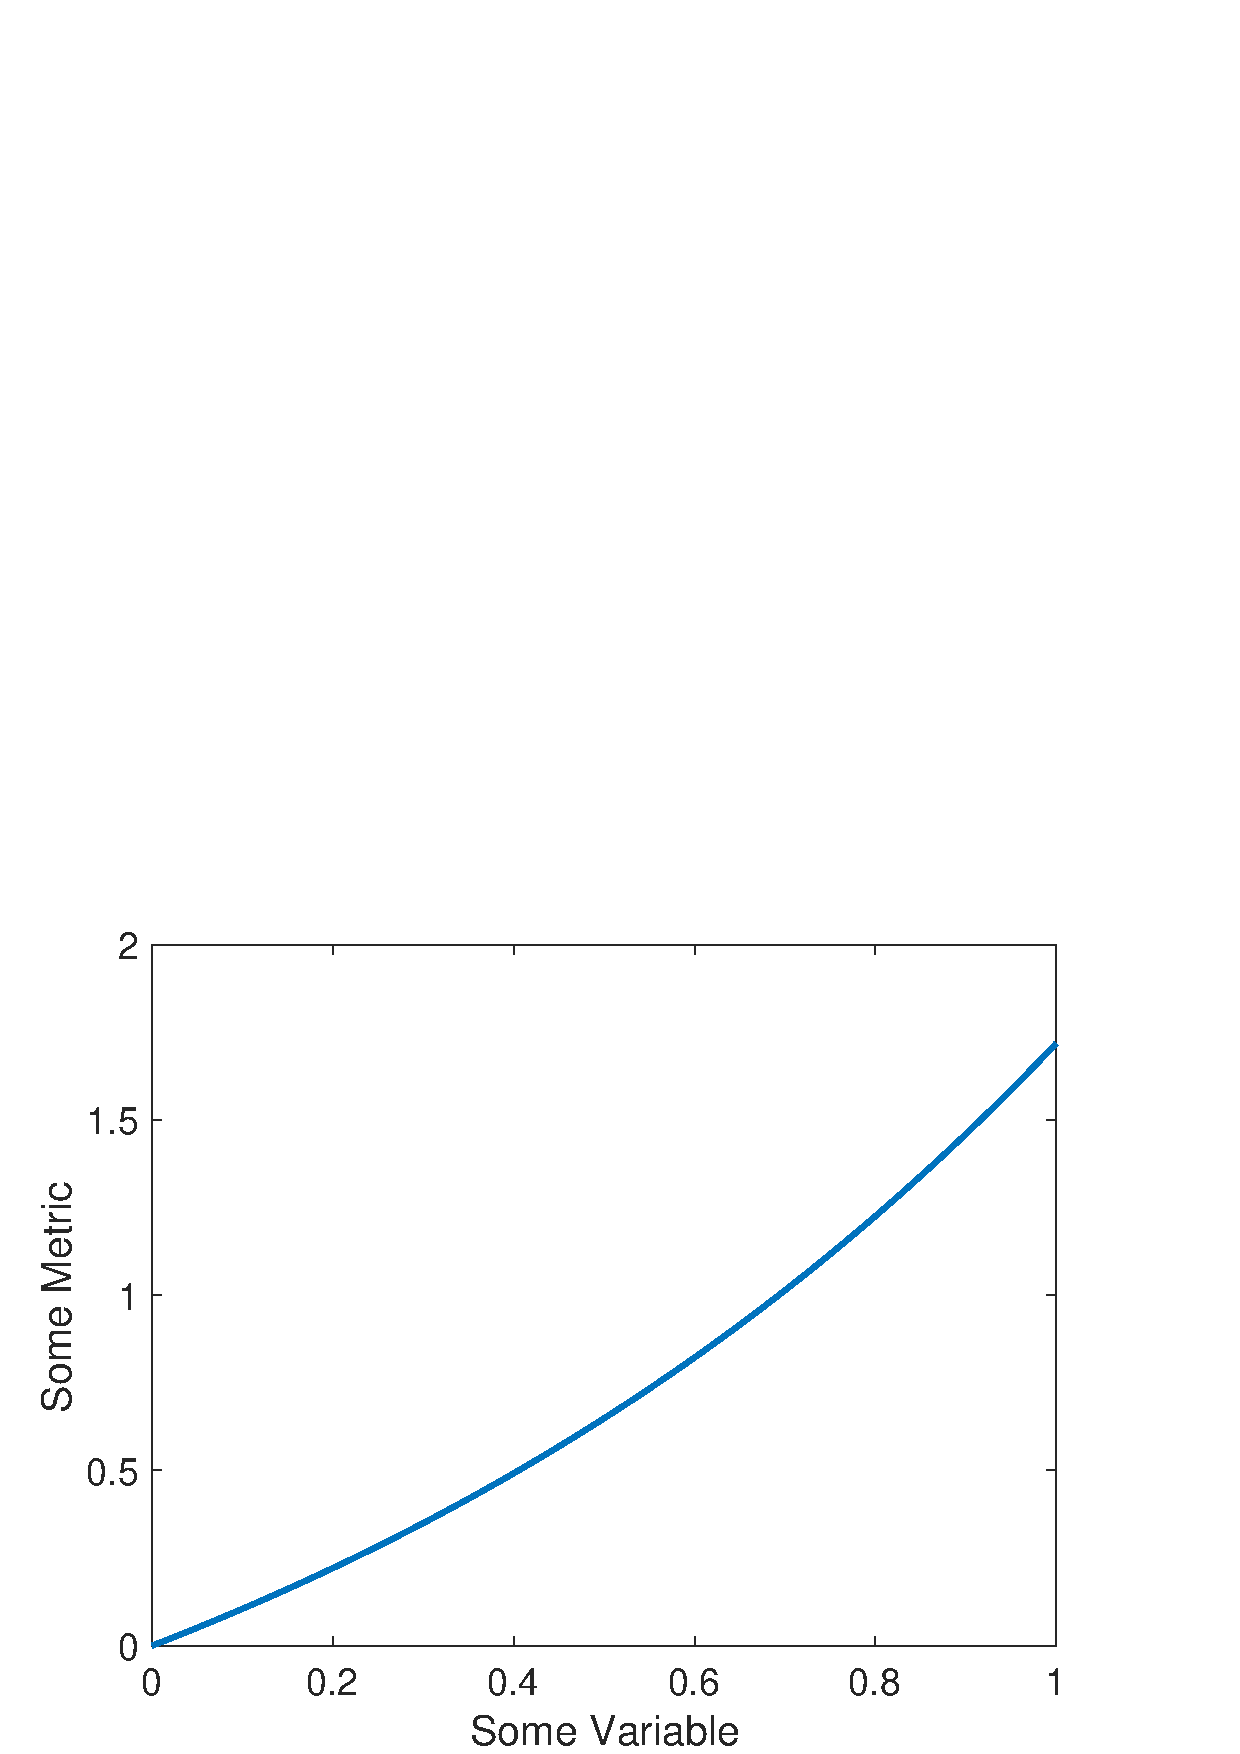
\includegraphics[width=0.65\textwidth]{Images/a_graph.jpg}
            \caption{A bad JPEG graph exported from MATLAB.}
            \label{fig:BadGraph}
        \end{figure}
    
        When you make plots in MATLAB make sure you export them as EPS images and that the text and lines are of sufficient size to be seen in the final document, as in \Cref{fig:BetterGraph}.

        \begin{figure}[ht!]
            \centering
            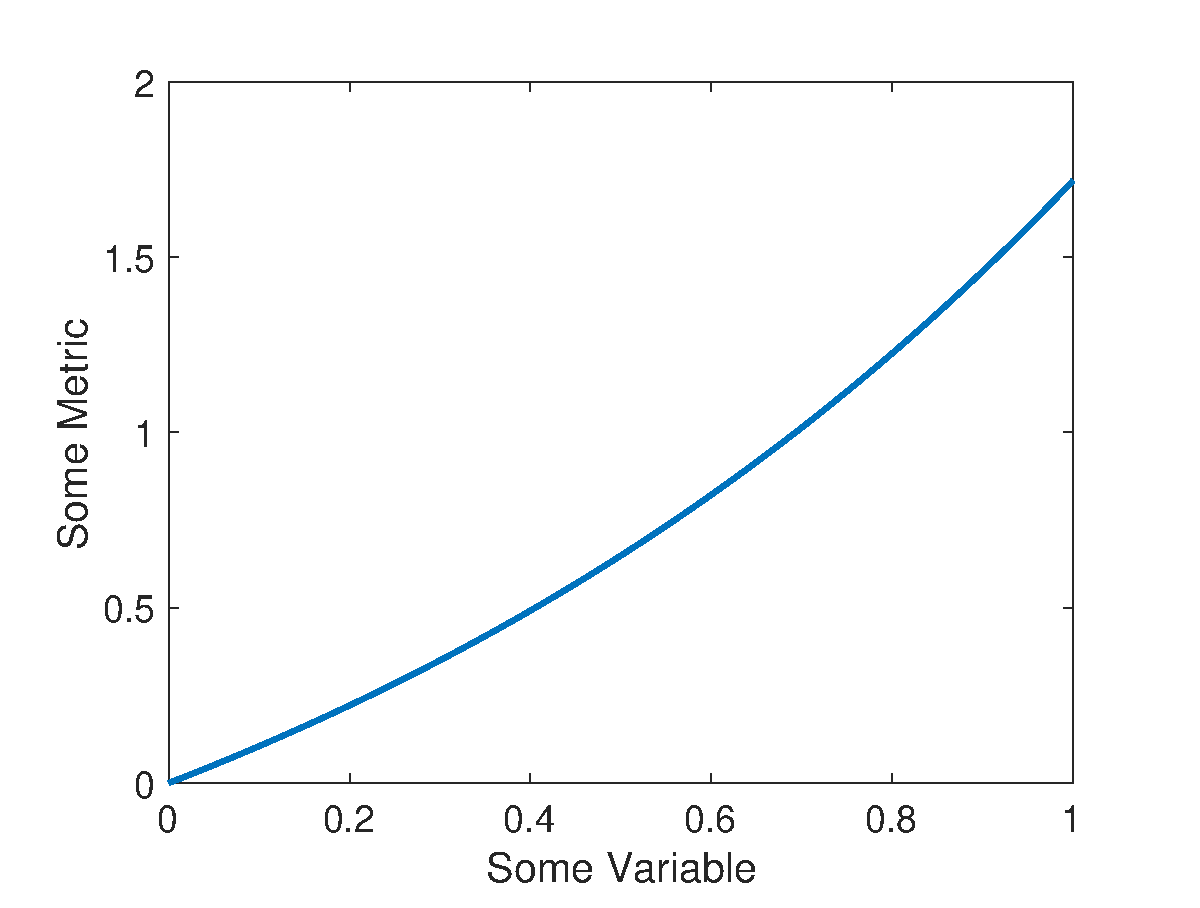
\includegraphics[width=0.65\textwidth]{Images/a_graph.eps}
            \caption{A better EPS graph exported from MATLAB.}
            \label{fig:BetterGraph}
        \end{figure}
    
    \subsection{Tables}
    \label{sec:Tables}
        You quite often need to limit the width of tables in your document. Latex provides the paragraph column type for this. But if you want things centre aligned you can use the additional column type provided by this template. See \Cref{tab:ColumnTypes} for a demonstration.
    
        \begin{table}[ht!]
            \centering
            \begin{tabular}{|p{4cm}|C{4cm}|}
                \hline
                The `p' column type produces a left aligned paragraph of the given width. & The `C' column type does the same but centre aligned. \tabularnewline
                \hline
            \end{tabular}
            \caption{Defining the width of table columns.}
            \label{tab:ColumnTypes}
        \end{table}
    
        There are several other fancy packages for doing tables in latex, so have a look around for what you need.

\end{appendices}

\end{document}